\chapter{Segmentation (Clustering)}

\begin{Definition}[Clustering]
Organiser les données en \textbf{groupes (clusters)} de sorte que les données
\textbf{similaires} soient ensemble. C'est de l'apprentissage \textbf{non supervisé} :
\textbf{les classes sont inconnues}, on les découvre.
\end{Definition}

\begin{Astuce}[: ce qu'est un \og bon \fg{} clustering]
\textbf{Forte similarité \emph{intra}-classe} (les points d'un même groupe se ressemblent)
\textbf{et faible similarité \emph{inter}-classes} (les groupes sont bien séparés).
\end{Astuce}

\section{Mesurer la qualité d'un cluster}
Chaque cluster $C_k$ ($N_k$ points) est caractérisé par :
\[ \text{centre de gravité } \mu_k=\frac{1}{N_k}\sum_{x_i\in C_k} x_i, \qquad
   \text{inertie } J_k=\sum_{x_i\in C_k} d^2(x_i,\mu_k). \]
\textbf{Inertie intra} (faible $=$ points concentrés autour du centre) ; \textbf{inertie inter}
(grande $=$ centres éloignés, clusters bien séparés). \textbf{Objectif :} minimiser l'intra et
maximiser l'inter.

\section{Clustering hiérarchique}
On construit un \textbf{dendrogramme} (arbre binaire de groupes). On le \textbf{coupe}
horizontalement pour obtenir le nombre de groupes voulu.
\begin{itemize}[leftmargin=1.4em,nosep]
  \item \textbf{Ascendant (agglomératif)} — le plus courant : on part de $n$ singletons et on
        \textbf{fusionne} les groupes les plus proches jusqu'à un seul groupe.
  \item \textbf{Descendant (divisif)} : on part d'un groupe et on le divise.
\end{itemize}
\textbf{Distance entre groupes} : \textbf{lien simple} (min des distances), \textbf{lien complet}
(max), \textbf{lien moyen} (moyenne).

\subsection{Exercice résolu — lien simple}
Matrice de distance :
\begin{center}\small
\begin{tabular}{c|cccc}
 & B & C & D & E\\\hline
A & 1 & 3 & 2 & 4\\
B &   & 3 & 2 & 3\\
C &   &   & 1 & 3\\
D &   &   &   & 5\\
\end{tabular}
\end{center}

\begin{Calcul}[: fusions successives (lien simple = min)]
\textbf{Étape 1} : plus petite distance $=1$ pour $(A,B)$ et $(C,D)$. On fusionne
$\mathbf{\{A,B\}}$ (distance 1). Mise à jour (min) :
$d(\{A,B\},C)=\min(3,3)=3$, $d(\{A,B\},D)=\min(2,2)=2$, $d(\{A,B\},E)=\min(4,3)=3$.\\[3pt]
\textbf{Étape 2} : plus petite $=d(C,D)=1$ $\rightarrow$ fusion $\mathbf{\{C,D\}}$. Mise à jour :
$d(\{A,B\},\{C,D\})=\min(3,2)=2$, $d(\{C,D\},E)=\min(3,5)=3$.\\[3pt]
\textbf{Étape 3} : plus petite $=d(\{A,B\},\{C,D\})=2$ $\rightarrow$ fusion
$\mathbf{\{A,B,C,D\}}$. Reste $d(\{A,B,C,D\},E)=\min(3,3)=3$.\\[3pt]
\textbf{Étape 4} : fusion finale avec $E$ à la hauteur \textbf{3}.
\end{Calcul}

\begin{Exemple}[dendrogramme]
Hauteurs de fusion : $\{A,B\}$ et $\{C,D\}$ à $\mathbf{1}$, puis $\{AB,CD\}$ à $\mathbf{2}$,
puis $\{ABCD,E\}$ à $\mathbf{3}$. En coupant à hauteur $2{,}5$ on obtient \textbf{2 groupes} :
$\{A,B,C,D\}$ et $\{E\}$.
\end{Exemple}

\begin{Astuce}[: et avec un autre lien ? (comparaison sur la même matrice)]
Le \emph{lien} change la façon de mesurer la distance entre groupes, donc les hauteurs de
fusion. Sur la même matrice :
\begin{center}\small
\renewcommand{\arraystretch}{1.25}
\begin{tabular}{l l}
\toprule
Lien & Fusions (groupe @ hauteur)\\
\midrule
\textbf{Simple} (min) & $\{AB\}@1,\ \{CD\}@1,\ \{ABCD\}@\mathbf{2},\ \{ABCDE\}@\mathbf{3}$\\
\textbf{Complet} (max) & $\{AB\}@1,\ \{CD\}@1,\ \{ABCD\}@\mathbf{3},\ \{ABCDE\}@\mathbf{5}$\\
\bottomrule
\end{tabular}
\end{center}
Détail du \emph{lien complet} (on prend le \emph{max}) : après $\{A,B\}$ et $\{C,D\}$,
$d(\{A,B\},\{C,D\})=\max(3,2,3,2)=3$ (au lieu de $2$), et la dernière fusion avec $E$ se fait
à $\max(4,3,3,5)=5$ (au lieu de $3$). Le lien complet donne des clusters plus \og compacts \fg{},
le lien simple peut produire des \og chaînes \fg{} allongées.
\end{Astuce}

\begin{figure}[ht]\centering
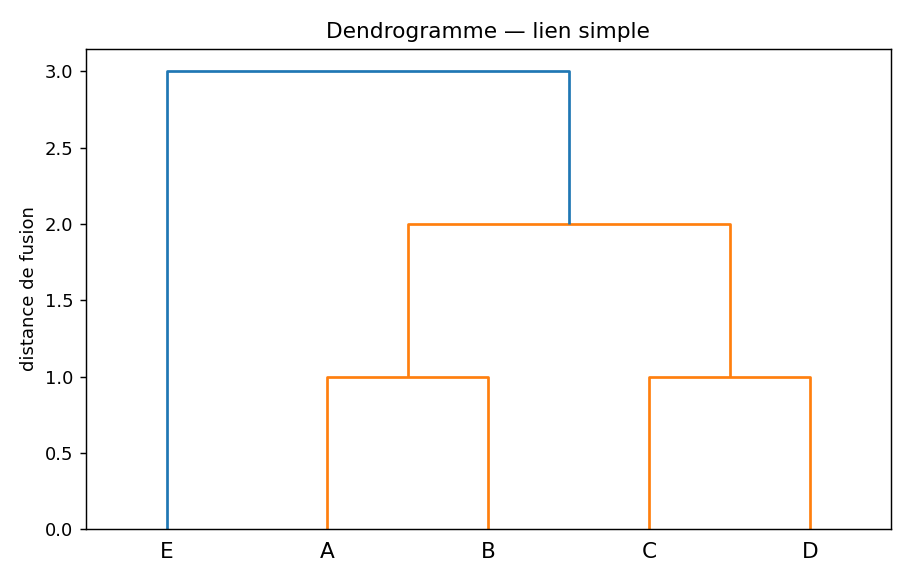
\includegraphics[width=0.55\linewidth]{figures/hierarchique_dendrogramme.png}
\caption{Dendrogramme (lien simple) obtenu avec SciPy — cohérent avec le calcul à la main.}
\end{figure}

\lstinputlisting[caption={scripts/hierarchique\_lien\_simple.py},label=lst:hier]{../scripts/hierarchique_lien_simple.py}

\section{Clustering par partitionnement — K-means}

\begin{Definition}[K-means]
On fixe $K$ à l'avance. On alterne deux étapes jusqu'à convergence :
\textbf{(1) Affectation} — chaque point va au centre $\mu_\ell$ le plus proche ;
\textbf{(2) Mise à jour} — chaque centre devient la \emph{moyenne} de son cluster.
Critère d'arrêt : les centres ne bougent plus,
$\sum_i \|\mu_i^{t}-\mu_i^{t-1}\|^2 \le \epsilon$.
\end{Definition}

\subsection{Exercice résolu — $C=\{2,3,4,10,11,12,20,25,30\}$, $K=2$, $\mu_1=2,\mu_2=4$}

À chaque itération : pour chaque point on compare $|x-\mu_1|$ et $|x-\mu_2|$, on l'affecte au
plus petit ; puis on recalcule chaque centre comme \emph{moyenne} de son groupe.

\begin{Calcul}[: itération 1 en entier ($\mu_1{=}2,\mu_2{=}4$)]
\begin{center}\small
\begin{tabular}{ccccc}
\toprule
$x$ & $|x-2|$ & $|x-4|$ & le plus proche & groupe\\
\midrule
2 & 0 & 2 & $\mu_1$ & $C_1$\\
3 & 1 & 1 & égalité $\to\mu_1$ & $C_1$\\
4 & 2 & 0 & $\mu_2$ & $C_2$\\
10,11,12,20,25,30 & grand & moins grand & $\mu_2$ & $C_2$\\
\bottomrule
\end{tabular}
\end{center}
$C_1=\{2,3\}\to\mu_1=\tfrac{2+3}{2}=2{,}5$ ;\quad
$C_2=\{4,10,11,12,20,25,30\}\to\mu_2=\tfrac{112}{7}=16$.
\end{Calcul}

\begin{Calcul}[: itérations 2 à 5 (résumé des recalculs)]
\textbf{It.\ 2} ($2{,}5;16$) : $C_1=\{2,3,4\}\to\mu_1=3$ ; $C_2=\{10,\dots,30\}\to\mu_2=18$.\\
\textbf{It.\ 3} ($3;18$) : $10$ bascule en $C_1$ car $|10-3|=7<|10-18|=8$.
$C_1=\{2,3,4,10\}\to\mu_1=4{,}75$ ; $C_2=\{11,12,20,25,30\}\to\mu_2=19{,}6$.\\
\textbf{It.\ 4} ($4{,}75;19{,}6$) : $11$ et $12$ basculent en $C_1$ ($|12-4{,}75|=7{,}25<|12-19{,}6|=7{,}6$).
$C_1=\{2,3,4,10,11,12\}\to\mu_1=7$ ; $C_2=\{20,25,30\}\to\mu_2=25$.\\
\textbf{It.\ 5} ($7;25$) : aucune réaffectation, mêmes moyennes $\Rightarrow$
\textbf{convergence} ($\sum_i\|\mu_i^{t}-\mu_i^{t-1}\|^2=0\le\epsilon$).
\end{Calcul}

\begin{Exemple}[résultat]
$\boxed{C_1=\{2,3,4,10,11,12\}\ (\text{centre }7) \qquad C_2=\{20,25,30\}\ (\text{centre }25)}$
\end{Exemple}

\begin{Calcul}[: qualité finale — l'inertie (intra-cluster)]
$J_k=\sum_{x\in C_k}(x-\mu_k)^2$ mesure la dispersion d'un cluster autour de son centre.
\begin{align*}
J_1 &=(2{-}7)^2+(3{-}7)^2+(4{-}7)^2+(10{-}7)^2+(11{-}7)^2+(12{-}7)^2=25{+}16{+}9{+}9{+}16{+}25=100\\
J_2 &=(20{-}25)^2+(25{-}25)^2+(30{-}25)^2=25{+}0{+}25=50
\end{align*}
\textbf{Inertie totale} $J=J_1+J_2=\mathbf{150}$. C'est exactement le \emph{within-cluster
sum of squares} affiché par scikit-learn (\texttt{inertia\_}) et par WEKA. Plus elle est
faible, plus les clusters sont \og serrés \fg{}.
\end{Calcul}

\begin{figure}[ht]\centering
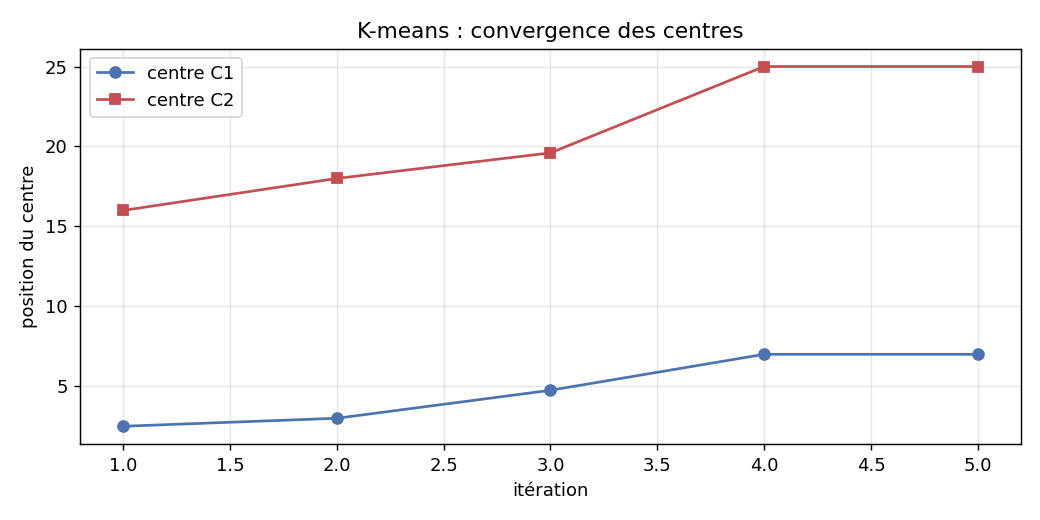
\includegraphics[width=0.49\linewidth]{figures/kmeans_convergence.png}
\hfill
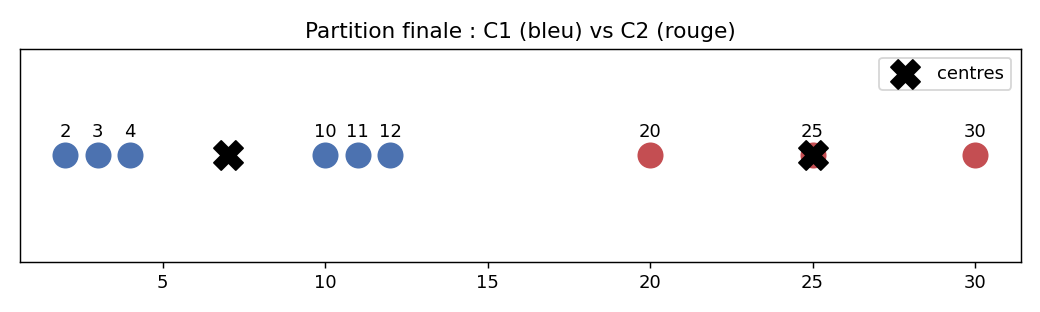
\includegraphics[width=0.49\linewidth]{figures/kmeans_partition.png}
\caption{À gauche : déplacement des centres au fil des itérations. À droite : partition finale.}
\end{figure}

\begin{Attention}
K-means dépend de l'\textbf{initialisation} des centres et exige des \textbf{distances}
(donc \textbf{normaliser} les attributs). Il faut aussi \textbf{choisir $K$} (méthode du coude,
silhouette\dots).
\end{Attention}

\lstinputlisting[caption={scripts/kmeans\_1d.py},label=lst:kmeans]{../scripts/kmeans_1d.py}

\begin{Resume}
\textbf{Hiérarchique} : fusions successives (lien simple/complet/moyen) $\rightarrow$
dendrogramme que l'on coupe. \textbf{K-means} : $K$ fixé, on alterne
affectation $\leftrightarrow$ recalcul des moyennes jusqu'à stabilité. Les deux cherchent
\textbf{forte cohésion interne} et \textbf{forte séparation} entre groupes.
\end{Resume}
